\section{Desarrollo en la MT3620}
Esta tablilla tiene dos tipos de aplicaciones que se le pueden desarrollar: la de alto nivel y la de tiempo real. A pesar de que sean dos tipos de implementación, estas se pueden desarrollar con total comodidad en la IDE que hayas elegido.


\subsection{Alto nivel}
Este tipo de aplicación es requerida en cada dispositivo Azure Sphere. El código corre en el sistema operativo de Azure Sphere. Puedes usar librerías de aplicaciones.

Estas pueden:
\begin{itemize}
	\item
	Configurar los periféricos de la Azure Sphere como el GPIO, UARTs y otras interfaces.
	\item 
	Comunicarse con las aplicaciones de tiempo real.
	\item 
	Comunicarse por medio del Internet.
\end{itemize}

Este es el uso normal del microcontrolador. Este tipo solo puede acceder a librerías que permita Microsoft, no tiene permitido el acceso mediante shell o archivos del I/O.

\subsection{Tiempo Real}
En este tipo de aplicación está más cerca del metal, por lo que en este puedes interactuar y configurar con los puertos del microcontrolador. También puedes implementar un sistema operativo en tiempo real y estas aplicaciones pueden comunicarse con las de alto nivel.

\section{Definiciones de hardware}
Desarrollar en este tipo de tarjetas de desarrollo tiene sus beneficios, uno de estos son las definiciones de hardware, estas definen la locación de los periféricos. Ayudan a una mejor compresión en el código, en estas tarjetas hay dos archivos para modificar esto, primero están los especificados por el fabricante, estos ya vienen en el SDK de la Azure Sphere en el directorio \textit{ProgramFiles(x86)\textbackslash Microsoft Azure Sphere SDK\textbackslash HardwareDefinitions} en Windows y \textit{/opt/azurespheresdk/HardwareDefinitions} en Linux. También existen las definiciones de aplicaciones especificas, estas se crean a partir de las especificadas por el fabricante y asignan identificadores que se usan de referencia, así el cambio de una tablilla a otra es más sencillo.
Estos archivos están escritos en json, y su formato es el siguiente.
\begin{lstlisting}[language = json, firstnumber=1]
{
	"Metadata": //Informacion sobre el archivo
	{
		"Type": "Azure Sphere Hardware Definition",
		"Version": 1
	},
	"Description": //Informacion sobre la tablilla o modulo
	{
		"Name": "<nombre de la tablilla o modulo>",
		"MainCoreHeaderFileTopContent": [
		"/* Copyright (c) <vendor name> Todos los derechos reservados.",
		" <Informacion de alguna licencia> */",
		"",
		"// This header contains the peripheral pinout definitions for
		the",
		"// <name of board or module>"
		]
	},
	"Imports" : [ {"Path": ""} //Direccion del archivo de definicion de hardware para definir sobre ella
	],
	"Peripherals": [ //Los perifericos que se van usar para la aplicacion
	{"Name": "<Nombre en el codigo>", "Type": "<Tipo de periferico>", "Mapping": "<El nombre del periferico en el archivo importado>", "Comment": "<Informacion a destacar>"},
	]
}
\end{lstlisting}

\subsection{Creando el encabezado}
Después de tener definidas los componentes a utilizar, se puede generar el archivo .h, en la terminal se pone el siguiente comando:
\begin{verbatim}
azsphere hardware-definition generate-header --hardware-definition-file
<filename> 
\end{verbatim}
\begin{figure}[h]
	\centering
	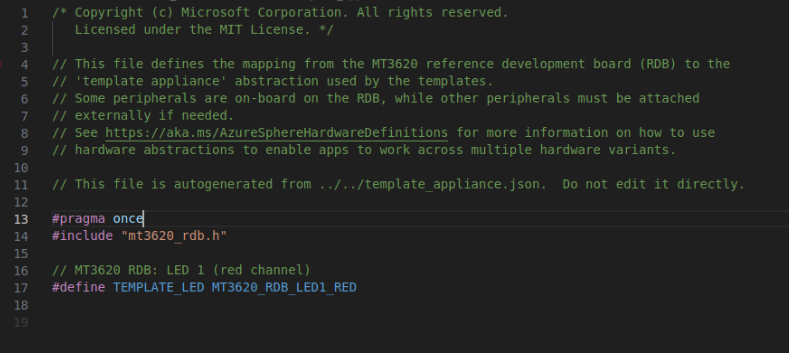
\includegraphics[width=\textwidth,height=\textheight,keepaspectratio]{header}
	\caption{Ejemplo de archivo header del proyecto blink}
\end{figure}

\textbf{Nota}: por defecto, el archivo encabezado creará una carpeta que siempre será el subdirectorio de la locación donde se encuentre el archivo JSON.
\subsection{Declaración de aplicación}
También conocido como las capacidades de aplicación, es un archivo que indica los recursos a utilizar de la aplicación, cada proyecto debe de tener uno. En esta deben estar todos los puertos y módulos que se van a utilizar de la tarjeta, los recursos se declaran basados en la definición de hardware que se explicó anteriormente. Esta declaración siempre se encuentra en el archivo app\_manifest.json
\begin{figure}[h]
	\centering
	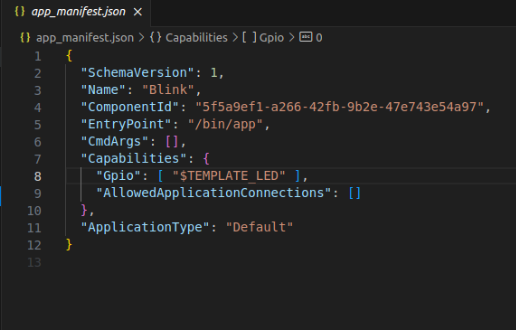
\includegraphics[scale=.60]{appmanifest}
	\caption{Ejemplo app\_manifest.json del proyecto blink}
\end{figure}
\subsection{Usando las definiciones del SDK}

\begin{enumerate}
	\item Se tiene que generar un proyecto en blanco, después en el archivo CMakeList.txt se anade la siguiente linea:
	\begin{verbatim}
	azsphere_target_hardware_definition(${PROJECT_NAME} 
	TARGET_DEFINITION "mt3620_rdb.json") 
	\end{verbatim}
	\item 
	En el archivo main.c incluir el archivo tipo cabecera correspondiente.
	\begin{lstlisting}[language = C, firstnumber=0]
#include  "hw/mt3620_rdb.h"
	\end{lstlisting}
	\item 
	Cambiar el application manifest anadiendo el periferico ha utilizar, por ejemplo para usar un GPIO, se pone lo siguiente
	\begin{lstlisting}[language = json, firstnumber=0]
"Capabilities": 
{  
	"Gpio": [ "$MT3620_RDB_LED1_RED" ] 
}
	\end{lstlisting}
	\item 
	Compilar el proyecto
\end{enumerate}

